% !TeX program = pdflatex
% Standalone source. Compile with pdfLaTeX; no external figures are required.
\documentclass[11pt,a4paper]{article}
\usepackage[margin=20mm]{geometry}
\usepackage[T1]{fontenc}
\usepackage{lmodern}
\usepackage{amsmath,amssymb,booktabs,array,xcolor,tikz,fancyhdr,hyperref,listings,pgfplots}
\usetikzlibrary{calc,arrows.meta}
\hypersetup{colorlinks=true,linkcolor=blue!50!black,urlcolor=blue!50!black}
\definecolor{accent}{HTML}{124E66}
\definecolor{pcol}{HTML}{A24021}
\definecolor{ncol}{HTML}{175A86}
\pagestyle{fancy}\fancyhf{}\fancyhead[L]{\small EE3032 / Fall 2017 / HW2}
\fancyhead[R]{\small CMOS logic}\fancyfoot[C]{\thepage}
\setlength{\headheight}{15pt}\setlength{\parindent}{0pt}\setlength{\parskip}{6pt}
\renewcommand{\arraystretch}{1.2}
\newcommand{\answer}[1]{\par\noindent\colorbox{accent!9}{\parbox{0.96\linewidth}{#1}}\par}
\newcommand{\AND}{\,}
\newcommand{\VDD}{V_{\mathrm{DD}}}
\newcommand{\VSS}{V_{\mathrm{SS}}}
% A conventional switch-level MOS symbol: continuous channel, insulated gate,
% and a gate bubble for pMOS. Bulk terminals are omitted, as explained below.
% Arguments: device id, x, y, gate literal, p or n. t/b are upper/lower terminals.
\newcommand{\MOS}[5]{
  \coordinate (#1) at (#2,#3);
  \coordinate (#1t) at ($(#1)+(0,.55)$);
  \coordinate (#1b) at ($(#1)+(0,-.55)$);
  \draw (#1t)--($(#1)+(0,.30)$)--($(#1)+(-.18,.30)$);
  \draw ($(#1)+(-.18,.34)$)--($(#1)+(-.18,-.34)$);
  \draw ($(#1)+(-.18,-.30)$)--($(#1)+(0,-.30)$)--(#1b);
  \draw ($(#1)+(-.35,.33)$)--($(#1)+(-.35,-.33)$);
  \def\type{#5}\def\ptype{p}
  \ifx\type\ptype
    \draw ($(#1)+(-.78,0)$)--($(#1)+(-.53,0)$);
    \draw ($(#1)+(-.465,0)$) circle (.065);
    \draw ($(#1)+(-.40,0)$)--($(#1)+(-.35,0)$);
  \else
    \draw ($(#1)+(-.78,0)$)--($(#1)+(-.35,0)$);
  \fi
  \node[anchor=east] at ($(#1)+(-.82,0)$) {$#4$};
  \node[anchor=west,font=\scriptsize] at ($(#1)+(.10,0)$) {#1};
}
% A transmission-gate instance; its two MOS devices are expanded on page 3.
\newcommand{\TG}[4]{
  \node[draw,rounded corners=1pt,minimum width=11mm,minimum height=6mm,
        fill=accent!5,font=\small] (#1) at (#2,#3) {$\mathrm{TG}_{#4}$};
}

\pgfplotsset{compat=1.18}
\lstset{basicstyle=\ttfamily\scriptsize,breaklines=true,frame=single,columns=fullflexible}
\begin{document}
\begin{center}{\LARGE\bfseries 2017 HW2}\\[4pt]{\large Slew, Elmore Delay, and Gate Capacitance}\\[4pt]{\small EE3032 / Introduction to VLSI Design}\end{center}
The supplied two-page handwritten answer was read first. All four original questions are answered below, with independently derived assumptions and an executable calculator. The circuit diagrams and calculations are independently reproducible.
\section*{1. Faster input rise makes output fall faster}
An initially low input turns the pMOS on and the nMOS off, so $V_{\rm out}\simeq\VDD$. As the input rises, the nMOS begins discharging $C_L$ when $V_{\rm in}>V_{tn}$, while the pMOS continues sourcing current until $V_{\rm in}\gtrsim\VDD-|V_{tp}|$.
\[
 C_L\frac{dV_{\rm out}}{dt}=I_p(V_{\rm in},V_{\rm out})-I_n(V_{\rm in},V_{\rm out}).
\]
The faster stimulus a brings the nMOS to strong drive sooner and cuts off the opposing pMOS sooner. The net discharge current $I_n-I_p$ becomes large earlier and the output traverses its 90\%--10\% interval more quickly. Stimulus b keeps both devices partly on for longer and initially gives a smaller nMOS overdrive. Thus its output has a longer fall time at the same load and transistor sizes. This is a finite-input-slew effect, not a change in capacitance.
\begin{center}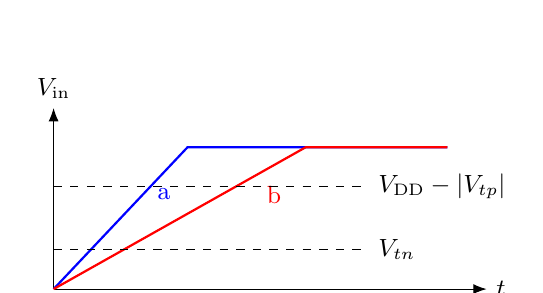
\begin{tikzpicture}[>=Latex,font=\small,x=1cm,y=1cm]
\draw[->] (0,0)--(5.5,0) node[right] {$t$};\draw[->] (0,0)--(0,2.3) node[above] {$V_{\rm in}$};
\draw[blue,thick] (0,0)--(1.7,1.8)--(5,1.8);\node[blue] at (1.4,1.2) {a};
\draw[red,thick] (0,0)--(3.2,1.8)--(5,1.8);\node[red] at (2.8,1.2) {b};
\draw[dashed] (0,.5)--(4,.5) node[right] {$V_{tn}$};\draw[dashed] (0,1.3)--(4,1.3) node[right] {$\VDD-|V_{tp}|$};
\end{tikzpicture}\end{center}
\textbf{Reference comparison.} The supplied answer correctly relates the quicker threshold crossings of a to faster discharge. We retain that explanation and make the opposing pull-up current explicit.
\section*{2. NAND followed by an inverter}
Use the prompt's effective on-resistance model and only the given total node capacitances $C_F,C_Z$. The internal NAND stack-node capacitance is not specified and is omitted in this two-node model. For the NAND output $F=\overline{AB}$, the worst pull-down traverses two nMOS in series, while the worst pull-up traverses only one pMOS:
\[
 \boxed{\tau_{F,HL}=2R_nC_F},\qquad
 \boxed{\tau_{F,LH}=R_pC_F}.
\]
For final output $Z=AB$, add the first-stage contribution and the inverter-stage contribution:
\[
 \boxed{\tau_{Z,LH}=2R_nC_F+R_pC_Z},\qquad
 \boxed{\tau_{Z,HL}=R_pC_F+R_nC_Z}.
\]
These are Elmore first-moment/time-constant estimates. If delay means an approximate 50\% crossing, use $t_{pd}\simeq\ln(2)\tau\simeq 0.693\tau$ consistently. A multistage nonlinear CMOS waveform is not a single exact exponential.
\newpage
The worst rising F transition is 11$\to$01 or 11$\to$10, with one active pMOS; 11$\to$00 turns both pMOS on in parallel and has a smaller effective $R_p/2$. F falling corresponds to an input transition into 11. Z changes in the opposite direction to F.
For a declared numerical example $R_n=1\,\mathrm{k}\Omega$, $R_p=2\,\mathrm{k}\Omega$, $C_F=10$ fF, and $C_Z=5$ fF:
\begin{center}\begin{tabular}{lrr}\toprule
Node/direction&Elmore $\tau$ (ps)&Approx. 50\% delay (ps)\\\midrule
F, H--L&20.000&13.863\\F, L--H&20.000&13.863\\
Z, H--L&25.000&17.329\\Z, L--H&30.000&20.794\\\bottomrule
\end{tabular}\end{center}
\textbf{Reference comparison.} The supplied answer introduces an additional stack-node capacitance $C_1$ and adds $R_nC_1$ in the NAND discharge term. That extension can be useful when $C_1$ is known, but the original prompt supplies only $C_F,C_Z$. We give the requested two-node expressions and state that internal-node parasitics require further data.
\section*{3. Mobility ratio at the inverter midpoint}
At $V_{\rm in}=V_{\rm out}=\VDD/2$, both devices are saturated for positive thresholds. Current equality gives
\[
 \frac{\mu_n C_{\rm ox}}2\,2\left(\frac{\VDD}2-V_{tn}\right)^2
 =\frac{\mu_p C_{\rm ox}}2\,4\left(\frac{\VDD}2-|V_{tp}|\right)^2.
\]
Therefore
\[
 \frac{\mu_n}{\mu_p}
 =2\left(\frac{\VDD/2-|V_{tp}|}{\VDD/2-V_{tn}}\right)^2,
 \qquad \boxed{\mu_n/\mu_p=2\ \text{if }V_{tn}=|V_{tp}|.}
\]
The value 2 is the intended matched-threshold square-law result and agrees with the reference. If threshold magnitudes differ, the midpoint condition alone does not determine a unique mobility ratio; the general expression above applies.
\section*{4. Capacitance at the fanout node x}
Ignoring wire/drain capacitance, node x drives one inverter input and one NOR input. Let the inverter gate capacitances be $C_n,C_p$, with $C_g=C_n+C_p$. The NOR must have the same worst-case nMOS pull-down strength and equivalent pMOS pull-up strength as the inverter. Thus each NOR nMOS has the inverter nMOS width, and each of its two series pMOS has twice the inverter pMOS width (same L).
\[
 C_{\rm NOR,pin}=C_n+2C_p,\qquad
 \boxed{C_x=C_g+C_{\rm NOR,pin}=2C_n+3C_p=2C_g+C_p.}
\]
\newpage
For a balanced inverter $\beta_n=\beta_p$ with $\mu_n=2\mu_p$, one needs $W_p=2W_n$. Since gate capacitance is proportional to $WL$, $C_p=2C_n$, giving
\[
 C_n=\frac 13C_g,\quad C_p=\frac 23C_g,\qquad
 \boxed{C_x=\frac 83 C_g}.
\]
\begin{center}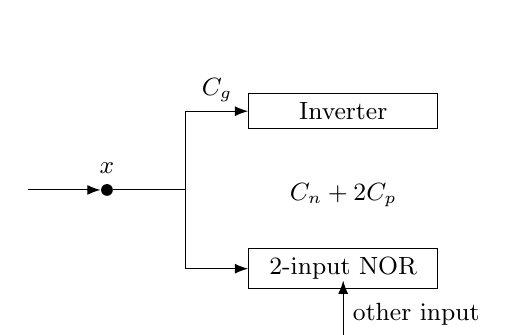
\begin{tikzpicture}[>=Latex,font=\small]
\node[circle,fill,inner sep=1.5pt,label=above:$x$] (x) at (0,0) {};
\node[draw,minimum width=24mm] (i) at (3,1) {Inverter};
\node[draw,minimum width=24mm] (n) at (3,-1) {2-input NOR};
\draw[->] (-1,0)--(x);\draw[->] (x)--(1,0)--(1,1)--(i.west) node[midway,above] {$C_g$};
\draw[->] (1,0)--(1,-1)--(n.west);
\node[above=4mm] at (n.north) {$C_n+2C_p$};
\draw[->] (3,-2)--(3,-1.15) node[midway,right] {other input};
\end{tikzpicture}\end{center}
\textbf{Assumption check.} The wording names $\beta_p,\beta_n$ separately; it does not explicitly equate them. With equal lengths but an unbalanced inverter, the general result is
\[
 \frac{C_x}{C_g}=\frac{2\beta_n+6\beta_p}{\beta_n+2\beta_p}
 \quad\text{for }\mu_n=2\mu_p.
\]
Consequently $8/3$ assumes the intended balanced reference inverter. The supplied answer uses that assumption and reaches the same result. The equal-equivalent-strength conditions for the NOR alone do not determine $\beta_p/\beta_n$.
\textbf{Reproduce.} \texttt{python verify\_design.py} evaluates every expression with declared parameters, exports \texttt{verification.json}, and checks the matched-threshold and balanced-inverter special cases. Use \texttt{--rn}, \texttt{--rp}, \texttt{--cf-ff}, \texttt{--cz-ff}, \texttt{--vtn}, \texttt{--vtp-abs}, and \texttt{--beta-p-over-n} to change the assumptions. These are analytical calculations, not fabricated HSPICE observations.
\end{document}
